\documentclass[crop,tikz,ifthenelse]{standalone}% 'crop' is the default for v1.0, before it was 'preview'
%\usetikzlibrary{...}% tikz package already loaded by 'tikz' option


\begin{document}
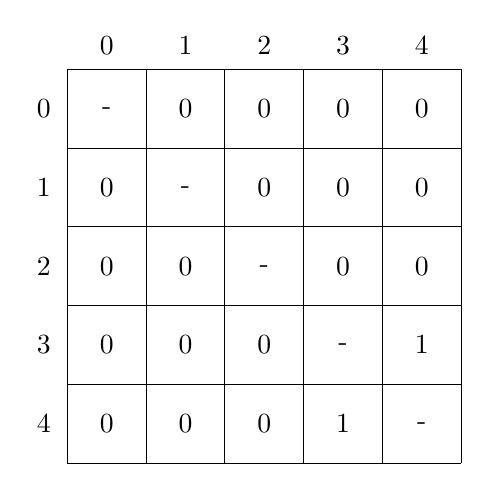
\begin{tikzpicture}[]

\newcommand{\wall}[2]{\filldraw[fill=black!30!white, draw=black] (#1,#2) rectangle (#1+1,#2+1);}
\newcommand{\area}[3]{\draw (#1,#2) rectangle (#1+1, #2+1) node[pos=.5] {#3};}
\newcommand{\door}[2]{\area{#1}{#2}{D};}
\newcommand{\player}[3]{\filldraw [fill=black, rotate around={#3:(#1,#2)}] (#1-0.5,#2-0.5) -- (#1,#2+0.5) -- (#1+0.5,#2-0.5) -- cycle;}
\newcommand{\enemy}[2]{\filldraw [fill=black] (#1,#2) circle(0.3) ;}


\foreach \x in {0,...,5}
  \draw (\x,5) -- (\x, 0);

\foreach \y in {0,...,5}
  \draw (0,\y) -- (5, \y);
  
  
\foreach \y in {0,...,4}
  \node at (-0.3, 4-\y+0.5) {\y} ; 

\foreach \x in {0,...,4}
  \node at (\x+0.5, 5.3) {\x} ; 

% bottom line
\node at (0.5, 0.5) {0} ; 
\node at (1.5, 0.5) {0} ; 
\node at (2.5, 0.5) {0} ; 
\node at (3.5, 0.5) {1} ; 
\node at (4.5, 0.5) {-} ; 

\node at (0.5, 1.5) {0} ; 
\node at (1.5, 1.5) {0} ; 
\node at (2.5, 1.5) {0} ; 
\node at (3.5, 1.5) {-} ; 
\node at (4.5, 1.5) {1} ;

\node at (0.5, 2.5) {0} ; 
\node at (1.5, 2.5) {0} ; 
\node at (2.5, 2.5) {-} ; 
\node at (3.5, 2.5) {0} ; 
\node at (4.5, 2.5) {0} ;

\node at (0.5, 3.5) {0} ; 
\node at (1.5, 3.5) {-} ; 
\node at (2.5, 3.5) {0} ; 
\node at (3.5, 3.5) {0} ; 
\node at (4.5, 3.5) {0} ;

% top line
\node at (0.5, 4.5) {-} ; 
\node at (1.5, 4.5) {0} ; 
\node at (2.5, 4.5) {0} ; 
\node at (3.5, 4.5) {0} ; 
\node at (4.5, 4.5) {0} ;
\end{tikzpicture}
\end{document}